\chapter{Theory}
\label{ch:theory}

\section{Rule 0 - No magic!}
\label{NoMagic}
Machine learning (ML) is an iterative process of improving a map between an input variable and an output target \cite{Maier2019}. In the case of medical image segmentation, initial model input corresponds to diagnostic patient images, and output to the ground truth segmentations created by an expert clinician\todo{or radiation therapist} \cite{Kazemifar_2018}. More generally, the map from input to output can be interpreted as a series of pattern recognition tasks (functions) used to automate decision making \cite{Maier2019}. `Training' a model involves repeated exposure to a large representative subset of all available data, and application of an optimisation algorithm designed to extract and select features that have predictive validity \cite{Maier2019}. For instance, if a vector $x\in\mathbb{R}^{n}$ is a complete representation of the features extracted by a model with parameters $\theta$ learned during the training phase, $\hat{y} = \hat{f}(\theta; x)$ is the prediction produced under the model $\hat{f}$.\footnote{Notation: $f(u; v)$ represents a function $f$ with variables $u$ evaluated at a fixed point $v$. For instance, in the initial input layer $v$ is the model input (CT image) upon which operators with parameters $u$ extract a feature map. This notation highlights that feature maps (also represented by $u$ when used as input in deeper layers) are dependent on the trainable model parameters $v$.} The primary decision-making unit of a neural network is the perceptron \cite{Maier2019}. Each perceptron includes a set of parameters $\theta = (w_{0}, ...,w_{n} )$, where $w_{0}$ is referred to as the activation bias, and $w = (w_{1},..,w_{n})$ as the weights. Together, these parameters perform a linear transformation $z = w \cdot x + w_{0}$\todo{put this equation in circle brackets?} of the input $x$. A single perceptron network has the modelling capacity of a binary classifier when combined with a smooth non-linear bounded monotonic function $h$ \cite{Maier2019}; i.e. $\hat{f}(\theta; x) = h(z)$ is the perceptron output or activation value of the node (`neuron'). Activation functions - historically a sigmoid function $\sigma(z)$ - ensure gradients are well defined during the optimisation process\todo{I thought the purpose of activation functions is so that the nueral network doesn't collapse to be the equivalent of a single layer due to the fact that a linear transformation of a linear transformation is equivalent to a single linear transformation. The non-linear function between the two linear transformations breaks this equivalence essentially allowing the creation of more than one layer in your nueral net.}, which iteratively improves model performance by comparing predicted output with the target output \cite{Maier2019}.

\begin{figure}[H]
	\begin{center}
		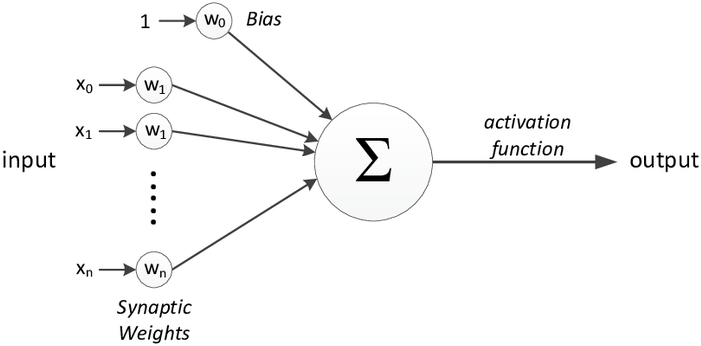
\includegraphics[width=0.7\textwidth]{perceptron}
		\caption{Single perceptron example with inputs x, trainable model parameters $\theta = (w_{0}, ...,w_{n} )$, and a non-linear activation function h. Output (or neuron activation value) is the `activated' linear combination $\hat{f}(\theta; x) = h(w \cdot x + w_{0})$ \cite{cintra2018}. Modified for notional consistency with this document.}
		\label{fig:percept}
	\end{center}
\end{figure}

From here, we already have the fundamental structure required to tell a student if they would pass or fail a subject without prior knowledge of assessment weighting
\todo{I'll leave this comment here, but I realised the question I provided probably wouldn't be able to be modelled by this case, as there is no means for inter pixel cross information. If you can think of a question that is true here, but still relevant to your thesis context that would be preferred, but if you can't think of something (I can't immediately) feel free to leave it. [OLD COMMENT START]Personally, this example could be equivalently presented, except instead the question could be ``is there a contour for this organ on this image''. By rewording the example to something relevant to your thesis it wouldn't feel so jarring. You can still make the same references as you are still describing a binary classifier as the output, and instead of test scores as input, the input is 262144x1 (512x512 in scanning order) pixel values.[/OLD COMMENT END]}
(i.e. a binary classifier for pass/fail) \cite{rosenblatt1957}. For instance, by exposing the model to enough past student assessment results $x$ and their final subject score $f(x)$, parameters of the perceptron $\theta$ can converge to an approximation of the true assessment weightings \cite{Lundervold2019}. Parameter convergence is achieved via a loss function which calculates the difference between target outputs $f(x)$ under the true map $f$, and the model predictions $\hat{f}(\theta; x)$ inferred from a `forward-pass' of the learned approximation $\hat{f}$ \cite{Bertels2019}. An optimisation algorithm minimises the loss $L(\theta) \sim |f(x)-\hat{f}(\theta; x)| \to 0$ with respect to $\theta$, while ensuring changes generalise to independent cases (i.e. new student data) from a validation dataset, sampled from the same distribution as the training data (i.e. same subject) \cite{Maier2019}. We note here that $L(\theta)$ is a user defined function to measure the difference between prediction and ground truth; and that the geometric norm was presented above for simplicity. Adjustment vectors (gradients) are calculated via the familiar differential operations of calculus (as seen in equation \ref{eq:calc}) \cite{Maier2019}.
\begin{equation}
\partial_{\theta} L = \partial_{\hat{f}}  L \; \partial_{\theta} \hat{f}
\label{eq:calc}
\end{equation}

Iterative parameter updates converge $L(\theta)$ to a local minimum via a first-order approximation (equation \ref{eq:forward}), commonly referred to as the gradient descent algorithm, where $\alpha>0$ is the step-size or `learning-rate' \cite{Maier2019}.
\begin{equation}
\theta^{i+1} = \theta^{i} - \alpha \partial_{\theta} L 
\label{eq:forward}
\end{equation}

However, it is only through the combination of multiple perceptrons that we can model non-linear decision boundaries \cite{Maier2019}. Literature has shown that a single layer multi-perception network is equivalent to an XOR operator \cite{Yanling}, and hence can approximate any continuous function on a closed and bounded Euclidean subset (i.e. compact subspace) of $\mathbb{R}^{n}$ \cite{Cybenko1989}. In multi-layer (indexed from $0$ to $n$) multi-perceptron arrangements (MLPs) i.e. $\hat{f}(\theta; x)= \hat{f}_{n}(\theta_{n};(\,... \,\hat{f}_{0}(\theta_{0}; x)))$, each neuron accepts activations from the previous layer as input - facilitating the emergence of complex decision-making processes and increased modelling capacity \cite{Maier2019}. In this case, the differential vector for loss (equation \ref{eq:calc}) must account for influence through multiple network pathways via the successive application of the chain rule (i.e. the back-propagation algorithm) \cite{Maier2019}. An additional complication arises from the fact that updates are usually averaged over a subset (mini-batch) of all available training data to reduce the computational burden (via stochastic gradient descent) \cite{Sun2019}; therefore, gradient calculations occur on an approximation of the true loss topology \cite{Sun2019}. Still, all we need is calculus, linear algebra, and some additional accounting - no magic!


\section{Going deeper with convolutional neural networks}
Convolutional neural networks (CNNs) are a subcategory of MLP networks, commonly used for deep learning concerning imaging tasks \cite{Maier2019}, where we can exploit the spatial relationship of input data to reduce complexity when compared to fully connected MLPs \cite{Lundervold2019}. Typical CNN operations consist of convolutional layers that perform feature extraction \cite{Hesamian2019}; as well as pooling layers responsible for feature selection via the sub-sampling of feature maps \cite{Ronneberger_2015}. Additionally, regularisation constraints (such as dropout layers) prevent over-fitting to the training data - a state by which features extracted under the model parameters (i.e. kernels in the case of CNNs) improve performance on the training data, yet fail to generalise to independent datasets \cite{Lundervold2019}. We provide a survey of each common layer type below, with visual context provided in Figure \ref{fig:convs}.

\begin{figure}[H]
	\begin{center}
		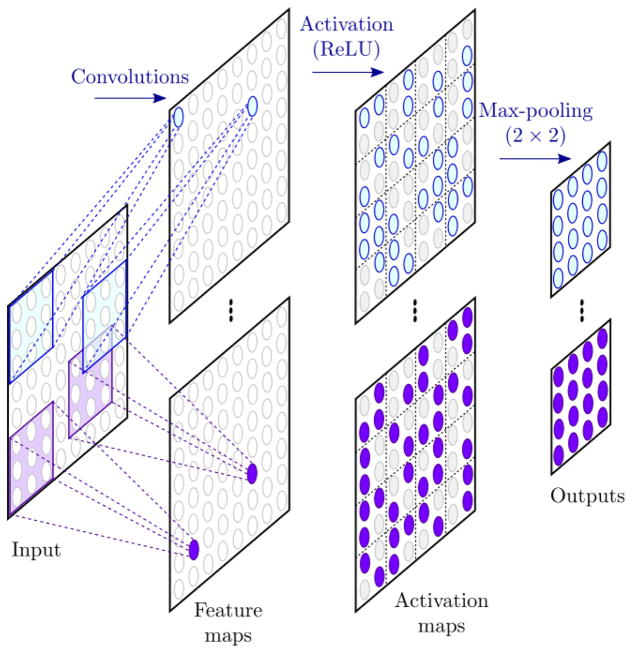
\includegraphics[width=0.65\textwidth]{convs}
		\caption{A typical sub-model arrangement seen in convolutional neural networks. Two 3 x 3 convolutional kernels (blue and purple) operate over the convolutional layer input. Each feature map has an associated kernel. The ReLU function performs non-linear activation on each extracted map. Finally, a 2 x 2 max-pooling layer halves the output dimensions and encodes a 2 x 2 translational in-variance for selected features in each partition \cite{Hesamian2019}.}
		\label{fig:convs}
	\end{center}
\end{figure}

\subsection{Convolution layers}
Each neuron (or node) in the feature maps receives input only from a restricted subsection of the previous layer (`local connectivity'), known as the receptive field, determined by the size of the convolutional kernel \cite{Hesamian2019}. A fundamental assumption of FCNs is that spatially close input neurons (i.e. input pixel values) have an increased significance for pattern recognition when compared to distant pixels \cite{Hu2015}. For instance, a 3 x 3 kernel will convolve around activation values from the previous layer, and each node in the output feature map will have a receptive field size of 9 pixels (3 x 3) corresponding to a location in the input. In the case of CNNs, filter values in each convolutional kernel are the model parameters; optimised to extract features with predictive validity during the back-propagation phase of training \cite{Maier2019}. It follows that larger filter sizes output single node values (and hence feature maps) that are representative of a spatially broader subset of information \cite{Nemoto_2020}. Each filter in a convolutional layer is associated with a feature representation of the input (known as a feature map) \cite{Hesamian2019}. In contrast to the fully connected perceptron networks described in section \ref{NoMagic}, a single filter convolves with the same kernel weights over the entire input domain - ensuring convolutional in-variance across an individual feature map \cite{Maier2019} - hence a specific pattern recognition task can be associated with each kernel in the layer \cite{Zeiler_2014}. In addition to making sense conceptually (i.e. edge detection is likely as useful over the entire input as it is on a kernel-sized subset), this `parameter sharing' has the added advantage of reducing the total number of parameters in a model; reducing both computational complexity and GPU memory requirements \cite{Lundervold2019}.\todo{Feel free to leave this as is, but it feels a little understated. The greater majority of custom neural network design is finding ways to reduce degrees of freedom in a sensible way. This convolutional nueral net allows for significantly deeper networks than what would be possible with the combinatorial explosion of a fully connected network. By limiting the connections to the relatively small number that will be of most help we make modern day nueral network training possible. CNNs are the first and foremost reason why machine learning for vision research is viable with today's hardware.}

\subsection{Pooling layers}
Pooling is a technique for sub-sampling feature maps in order to decrease resolution; and, to encode translational in-variance to activation values in its receptive field \cite{Lundervold2019}. For instance, a 2 x 2 max-pooling layer outputs the maximum value from each non-overlapping 2 x 2 grid partitioned from its input, halving the total feature map dimensions in the x-y plane, and encoding spatial in-variance with respect to the selected value over the 2 x 2 grid \cite{Lundervold2019}. Downsampling in this way is also possible via a 2D convolution with a stride size of 2. Convolutional pooling adds trainable parameters in the form of a kernel and has the benefit of simplifying the overall network structure due to the linear nature of convolution \cite{springenberg2014}.

\subsection{Dropout layers}
Dropout layers enforce a regularisation constraint by randomly sampling neurons in a network for deactivation; enforcing redundancy in a network, as adjusted architectures process each training batch \cite{Lundervold2019}. Weights are therefore optimised on multiple sub-variations of the complete network, resulting in stochastic averages with values sampled from a broad ensemble of networks \cite{srivastava2014}. Dropout layers improve generalisation and hence model performance when compared to fixed architectures. We note that dropout is deactivated during post-training inference, and predictions occur via the complete architecture \cite{Lundervold2019}.

\begin{figure}[H]
	\begin{center}
		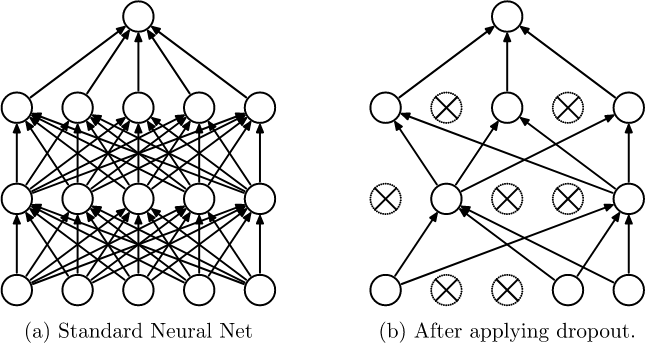
\includegraphics[width=0.65\textwidth]{dropout}
		\caption{Multi-layer perceptron with 2 hidden layers. (a) Standard network without dropout applied. (b) Standard network after applying dropout. The dropout technique randomly samples neurons in the network for deactivation, allowing parameter tuning to occur as averages over an ensemble of networks \cite{srivastava2014}.}
		\label{fig:dropout}
	\end{center}
\end{figure}

\subsection{Batch normalisation layers}
Batch normalisation layers are typically placed after activation layers (ordering is a topic of current research and alternative variations exist i.e. \cite{Kazemifar_2018}) to normalise activated feature maps. Hence, each batch normalisation layer adds two trainable parameters to the model, a mean and a variance value \cite{Lundervold2019}. Although batch normalisation has been shown to accelerate training and improve stability in layer distributions, its effectiveness is poorly understood from a theoretical perspective \cite{santurkar2018}. Conventional understanding states that batch normalisation penalises internal co-variance between network layers \cite{ioffe2015} and reduces effects of the vanishing/exploding gradient problems \cite{Li2014}. Additionally, parameter updates to feature maps in earlier layers are likely to significantly change the feature distribution of deeper layers - compounding internal variance in the optimisation process \cite{santurkar2018}. Hence, by normalising the output activation map, changes in layer distributions can be stabilised \cite{santurkar2018}. Conversely, studies have reported minimum improvements to internal co-variance under batch normalisation; and report that performance improvement is due to a smoothing of loss topology, which stabilises the behaviour of gradient descent \cite{santurkar2018}.

\subsection{Activation functions}
\label{sec:act}
In the previous section, we presented the fundamental structure of MLPs and expanded on this by examining CNN layers. However, `deep' learning is not possible with the typical sigmoid activation function presented in early MLP networks \cite{Lundervold2019} (included in equation \ref{eq:sigmoid}) due to the vanishing gradient problem - whereby multiple derivatives in the back-propagation algorithm with values $<1$ cause the loss gradient (equation \ref{eq:calc}) to decay exponentially as a function of the number of layers \cite{Lundervold2019}. 
\begin{equation}
\sigma(x) = \frac{1}{1+e^{-x}}
\label{eq:sigmoid}
\end{equation}

In contrast, convex functions such as the piecewise linear ReLU (Rectified linear unit - equation \ref{eq:ReLU}) have shown improved performance in deep layer arrangements due to the sparse nature of their activation \cite{Krizhevsky2012}; and, as non-saturating gradients prevent the vanishing gradient problem \cite{Lundervold2019}. However, contrary to activation function requirements stated in section \ref{NoMagic}, ReLU is neither smooth nor bounded, raising some technical challenges in its use \cite{Lundervold2019}. The unbounded nature of ReLU exposes the network to the well-known `exploding gradient problem' - as there is no constraint on activation values \cite{xu2015}. In addition, the `Dying ReLU problem` highlights a limitation associated with zeroing all negative activation inputs \cite{xu2015}. Zeroed activation values may fail to influence the loss function during gradient calculations; hence, this state partially prohibits parameter adjustment during training \cite{xu2015}. Although some recent CNN implementations attempt to offset the Dying ReLU problem via the so-called `Leaky ReLU' (which maintains a small non-zero gradient for activations $< 0$ \cite{Maas2013}), ReLU is still the default recommendation for most deep neural networks \cite{Goodfellow2016}.

\begin{equation}
ReLU(x) = max(0,x)
\label{eq:ReLU}
\end{equation}



%\todo[inline]{Addition?  Adam optimisation \cite{kingma2014} Probably not needed as not included in similar lit.}
%\section{Adam optimisation (Adaptive momentum)}
%Useful when rescaling learning rate 
%\begin{figure}[!htb]
%	\begin{center}
%		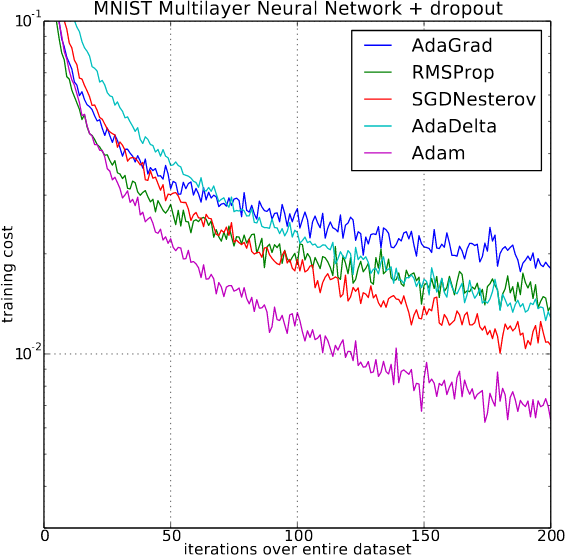
\includegraphics[width=0.45\textwidth]{adam}
%		\caption{Multi-layer perceptron with 2 hidden layers. (a) Standard network without dropout applied. (b) Standard network after applying dropout. The dropout technique randomly samples neurons in the network for deactivation, allowing parameter tuning to occur as averages over an ensemble of networks \cite{srivastava2014}.}
%		\label{fig:adam}
%	\end{center}
%\end{figure}

%
%\begin{equation}
%\theta^{i+1} = \theta^{i} + \alpha \partial_{\theta} L 
%\label{eq:BCE}
%\end{equation}
%
%\begin{equation}
%\theta^{i+1} = \theta^{i} + \alpha \partial_{\theta} L 
%\label{eq:softDSC}
%\end{equation}
%
%\begin{equation}
%\theta^{i+1} = \theta^{i} + \alpha \partial_{\theta} L 
%\label{eq:weightedsoftDSC}
%\end{equation}

%\subsection{Downsampling in U-net}
%\begin{figure}[!htb]
%	\begin{center}
%		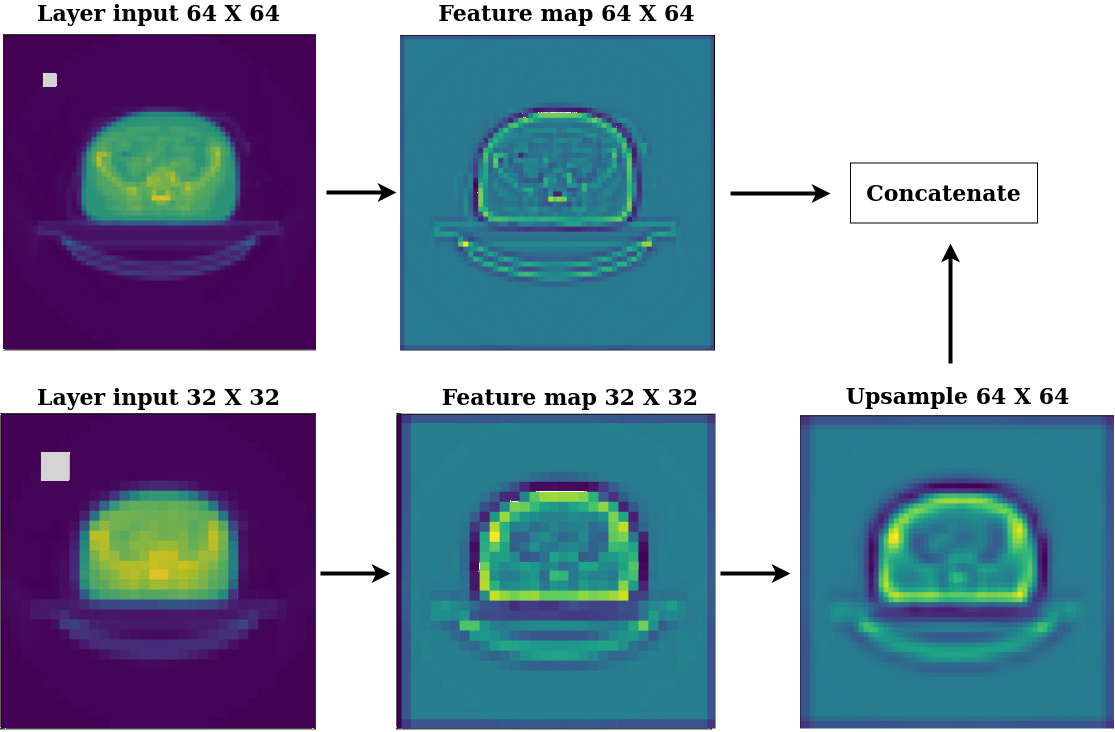
\includegraphics[width=1\textwidth]{figures/downsampling}
%		\caption{Edge detection shown over encoder-decoder pathway for multi-resolution analysis: Downsampling resolution increased the relative kernel size (grey - 3 x 3) to extract coarser (high level) image features for general localisation. Concatenate with high resolution features for local border segmentation}
%		\label{fig:downsampling}
%	\end{center}
%\end{figure}
